%------------------------------------------------------------
\chapter{テスト計算}\label{chap:test}
%------------------------------------------------------------

%------------------------------------------------------------
%------------------------------------------------------------
\section{流体力学}
%------------------------------------------------------------
%------------------------------------------------------------

%------------------------------------------------------------
\clearpage
\subsection{Sod解 (1次元)}
%------------------------------------------------------------

\begin{equation}
\left(
\begin{array}{c}
\rho_\mathrm{L} \\
v_\mathrm{L} \\
P_\mathrm{L} \\
\end{array}
\right)
= 
\left(
\begin{array}{c}
1 \\
0 \\
1 \\
\end{array}
\right),\;\;\;
\left(
\begin{array}{c}
\rho_\mathrm{R} \\
v_\mathrm{R} \\
P_\mathrm{R} \\
\end{array}
\right)
= 
\left(
\begin{array}{c}
0.125 \\
0 \\
0.1 \\
\end{array}
\right)
\end{equation}

図\ref{fig:laxhllhllc}左は、空間一次精度Lax法、HLL法、HLLC法
でSod解を解いた結果である。
Lax法では偶数番号と奇数番号のセルが
独立に時間発展するので、
いわゆるodd-even decouplingが起こる。
Lax法は、HLL法とHLLC法に比べ数値拡散が格段に多く入り、厳密解から大きくズレる。
Sod解ではHLL法とHLLC法に顕著な違いは見えないが、
$x=0.2$付近にある接触不連続面でHLLCの方が少しシャープになる。

図\ref{fig:laxhllhllc}右は、空間二次精度Lax法、HLL法、HLLC法
でSod解を解いた結果である。
HLL法とHLLC法は、厳密解に近い解が得られる。
Lax法ではodd-even decouplingのためにMUSCL法を使うと勾配が0に制限されてしまい、
一次精度になる。

\begin{figure}[htpb]
    \centering
    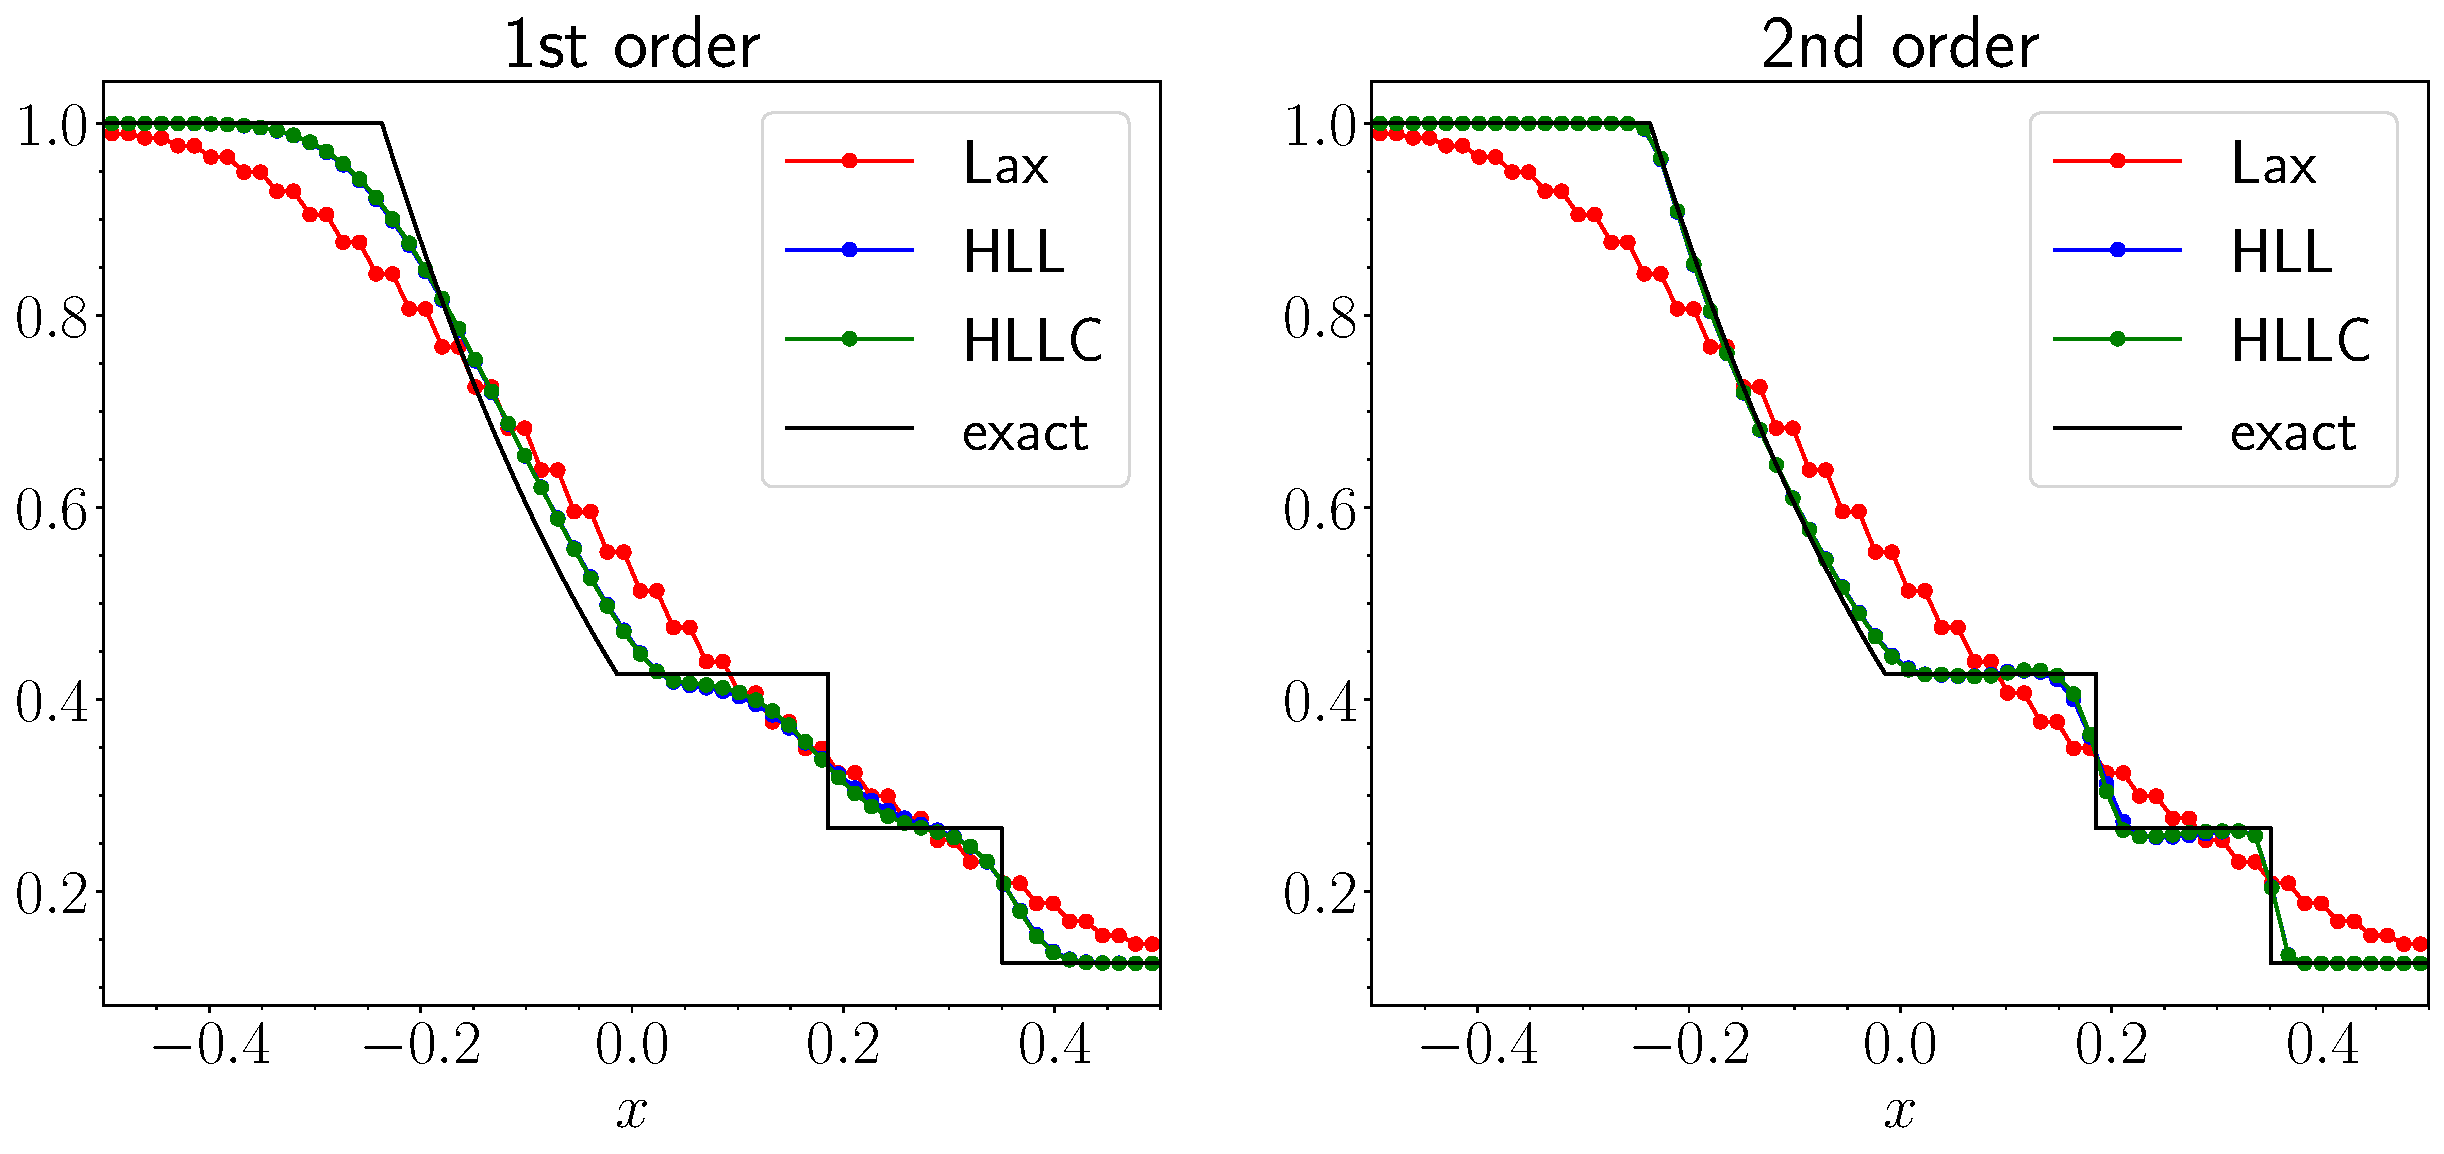
\includegraphics[width=10cm]{figures/sod_lax_hll_hllc.pdf}
    \caption{Sod解。Lax法、HLL法、HLLC法で解いた結果。
    左図が空間一次精度、右図が空間二次精度の結果。
    }
    \label{fig:laxhllhllc}
\end{figure}

%------------------------------------------------------------
\clearpage
\subsection{衝撃波管問題 (1次元)}
%------------------------------------------------------------

HLLとHLLCの結果の違いがより大きく出るように、
接触不連続面が動かない以下の衝撃波管問題を考える。
\begin{equation}
\left(
\begin{array}{c}
\rho_\mathrm{L} \\
v_\mathrm{L} \\
P_\mathrm{L} \\
\end{array}
\right)
= 
\left(
\begin{array}{c}
1 \\
1 \\
1 \\
\end{array}
\right),\;\;\;
\left(
\begin{array}{c}
\rho_\mathrm{R} \\
v_\mathrm{R} \\
P_\mathrm{R} \\
\end{array}
\right)
= 
\left(
\begin{array}{c}
0.25 \\
-2 \\
1 \\
\end{array}
\right)
\label{shini}
\end{equation}

この衝撃波管問題は左右から$x=0$向かって流体が衝突した結果、
$x=0$に接触不連続面ができ、$x<0$と$x>0$に2つの衝撃波が伝播する。
接触不連続面が$x=0$から動かない。
Sod解と同様に、Lax法は数値拡散が大きく、
解がほとんど再現できない。

この衝撃波管問題では移流による接触不連続面の数値拡散が入らないので、
HLL法とHLLC法の違いが顕著に見える。
接触不連続面はHLLCの方が格段によく捉えられている。


\begin{figure}[htpb]
    \centering
    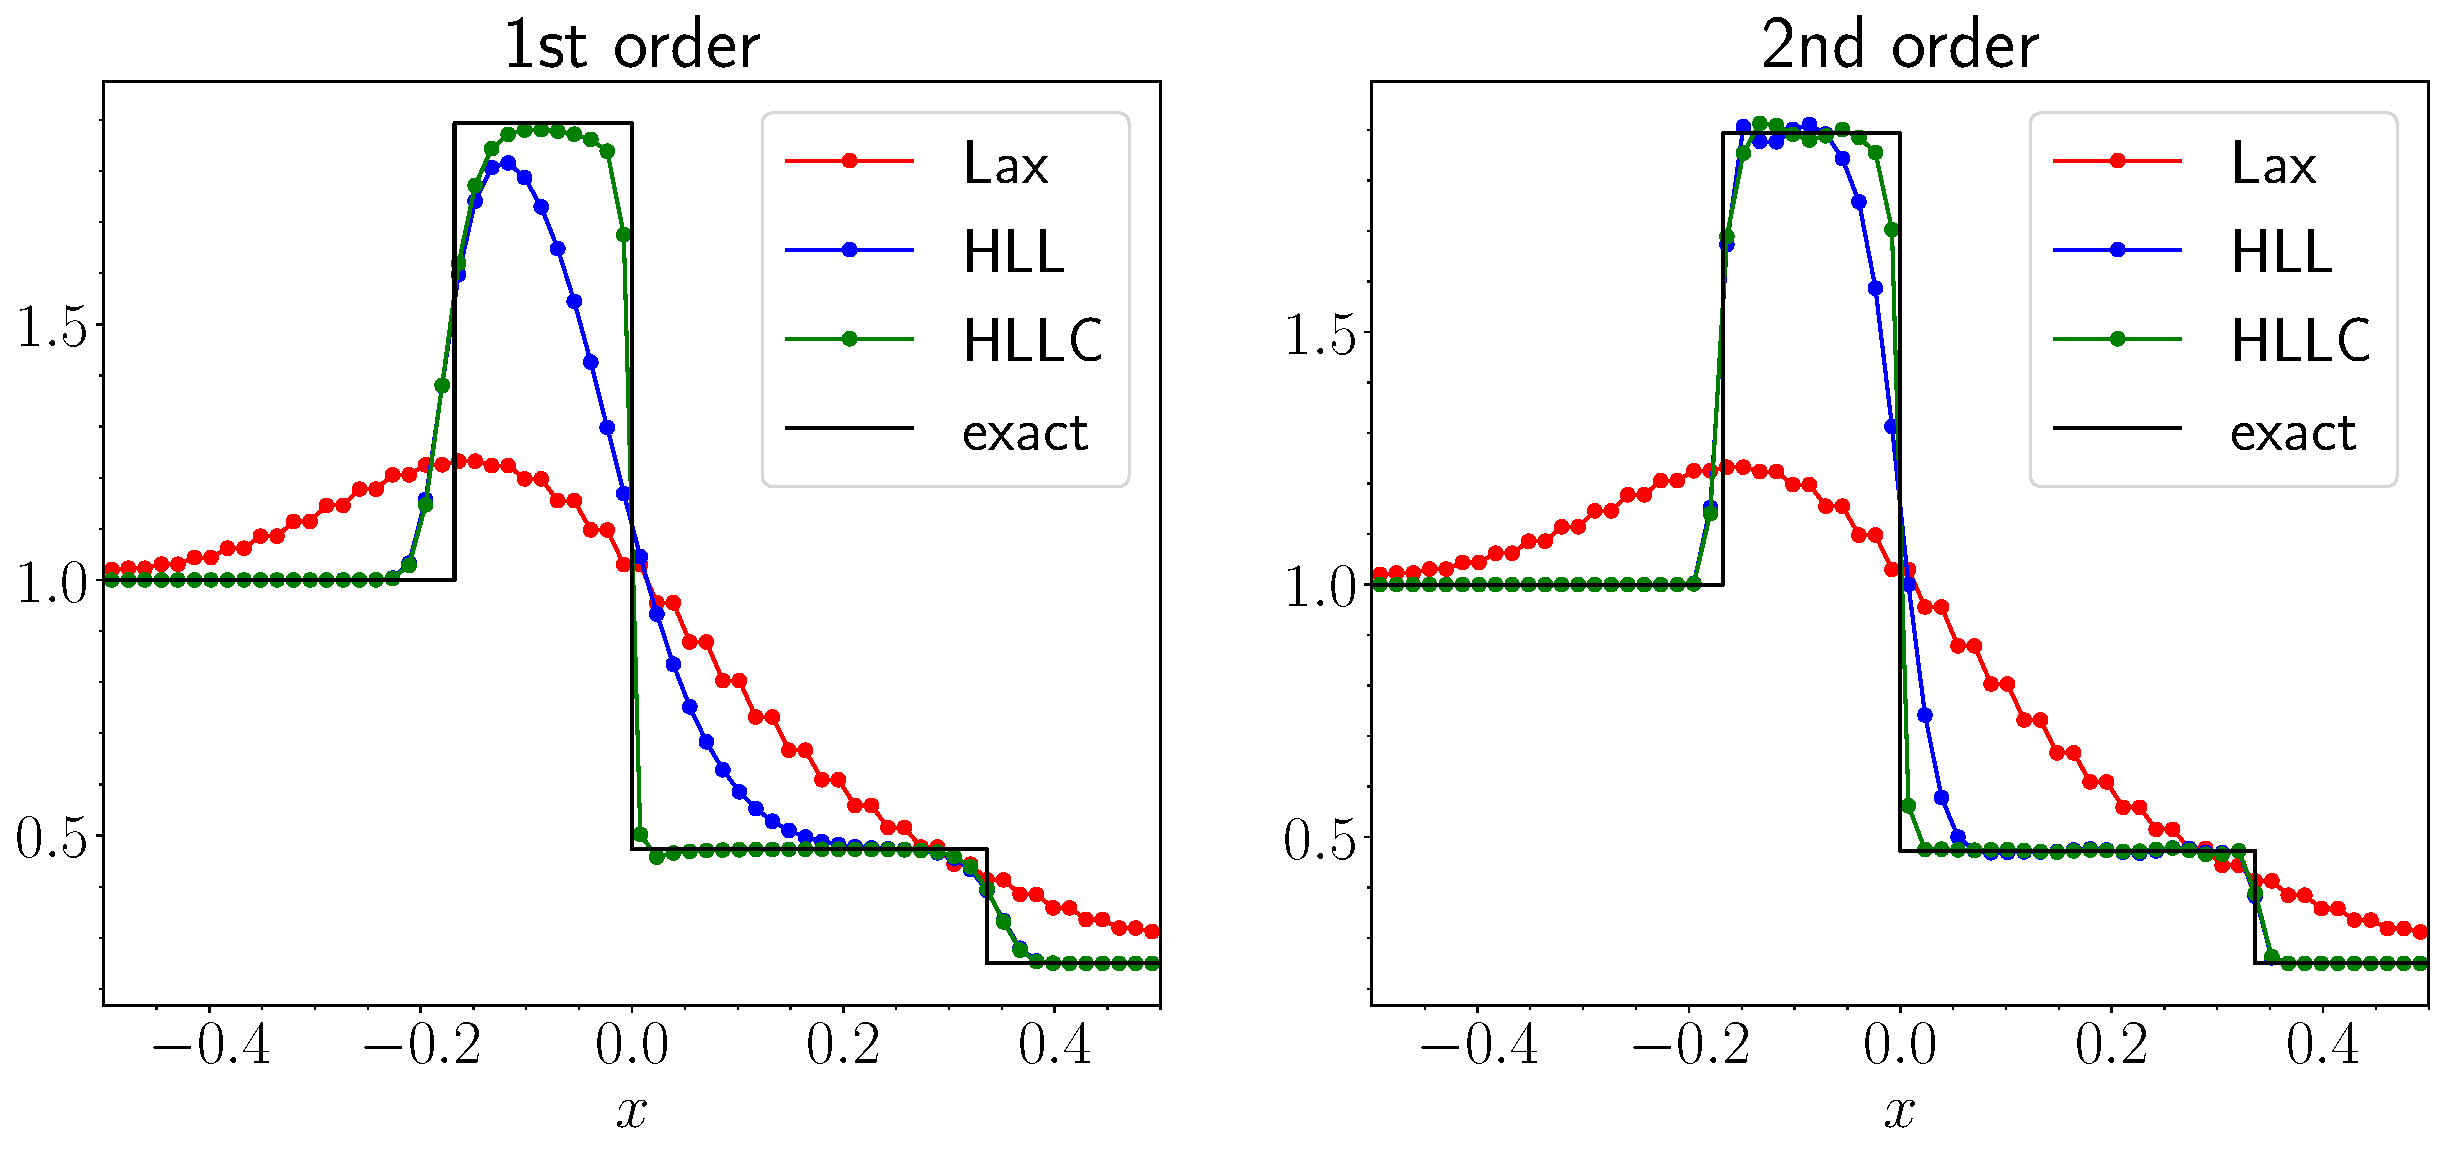
\includegraphics[width=10cm]{figures/sh_lax_hll_hllc.pdf}
    \caption{衝撃波管問題(初期条件は式\ref{shini})。Lax法、HLL法、HLLC法で解いた結果。
    左図が空間一次精度、右図が空間二次精度の結果。
    }
    \label{fig:laxhllhllc}
\end{figure}

%------------------------------------------------------------
\clearpage
\subsection{音波 (1次元)}
%------------------------------------------------------------

非摂動状態($\rho=1$、$v=0$、$P=1$)に、$+x$方向に伝播する音速を計算する。
\begin{equation}
\rho = 1 + 10^{-4}\sin(2\pi x),\;\;\;
v = 10^{-4}\sqrt{\gamma}\sin(2\pi x),\;\;\;
P = 1 + 10^{-4}\gamma \sin(2\pi x),\;\;\;
\end{equation}
1周期計算($1/\sqrt{\gamma}$)したあとに解析解との誤差を以下の式で測定する。
\begin{equation}
    \epsilon = \sqrt{ \frac{1}{N} \sum_{i=1}^N \left(\rho(x_i) - \rho_\mathrm{ana}(x_i)\right)^2}
\end{equation}

\begin{figure}[htpb]
    \centering
    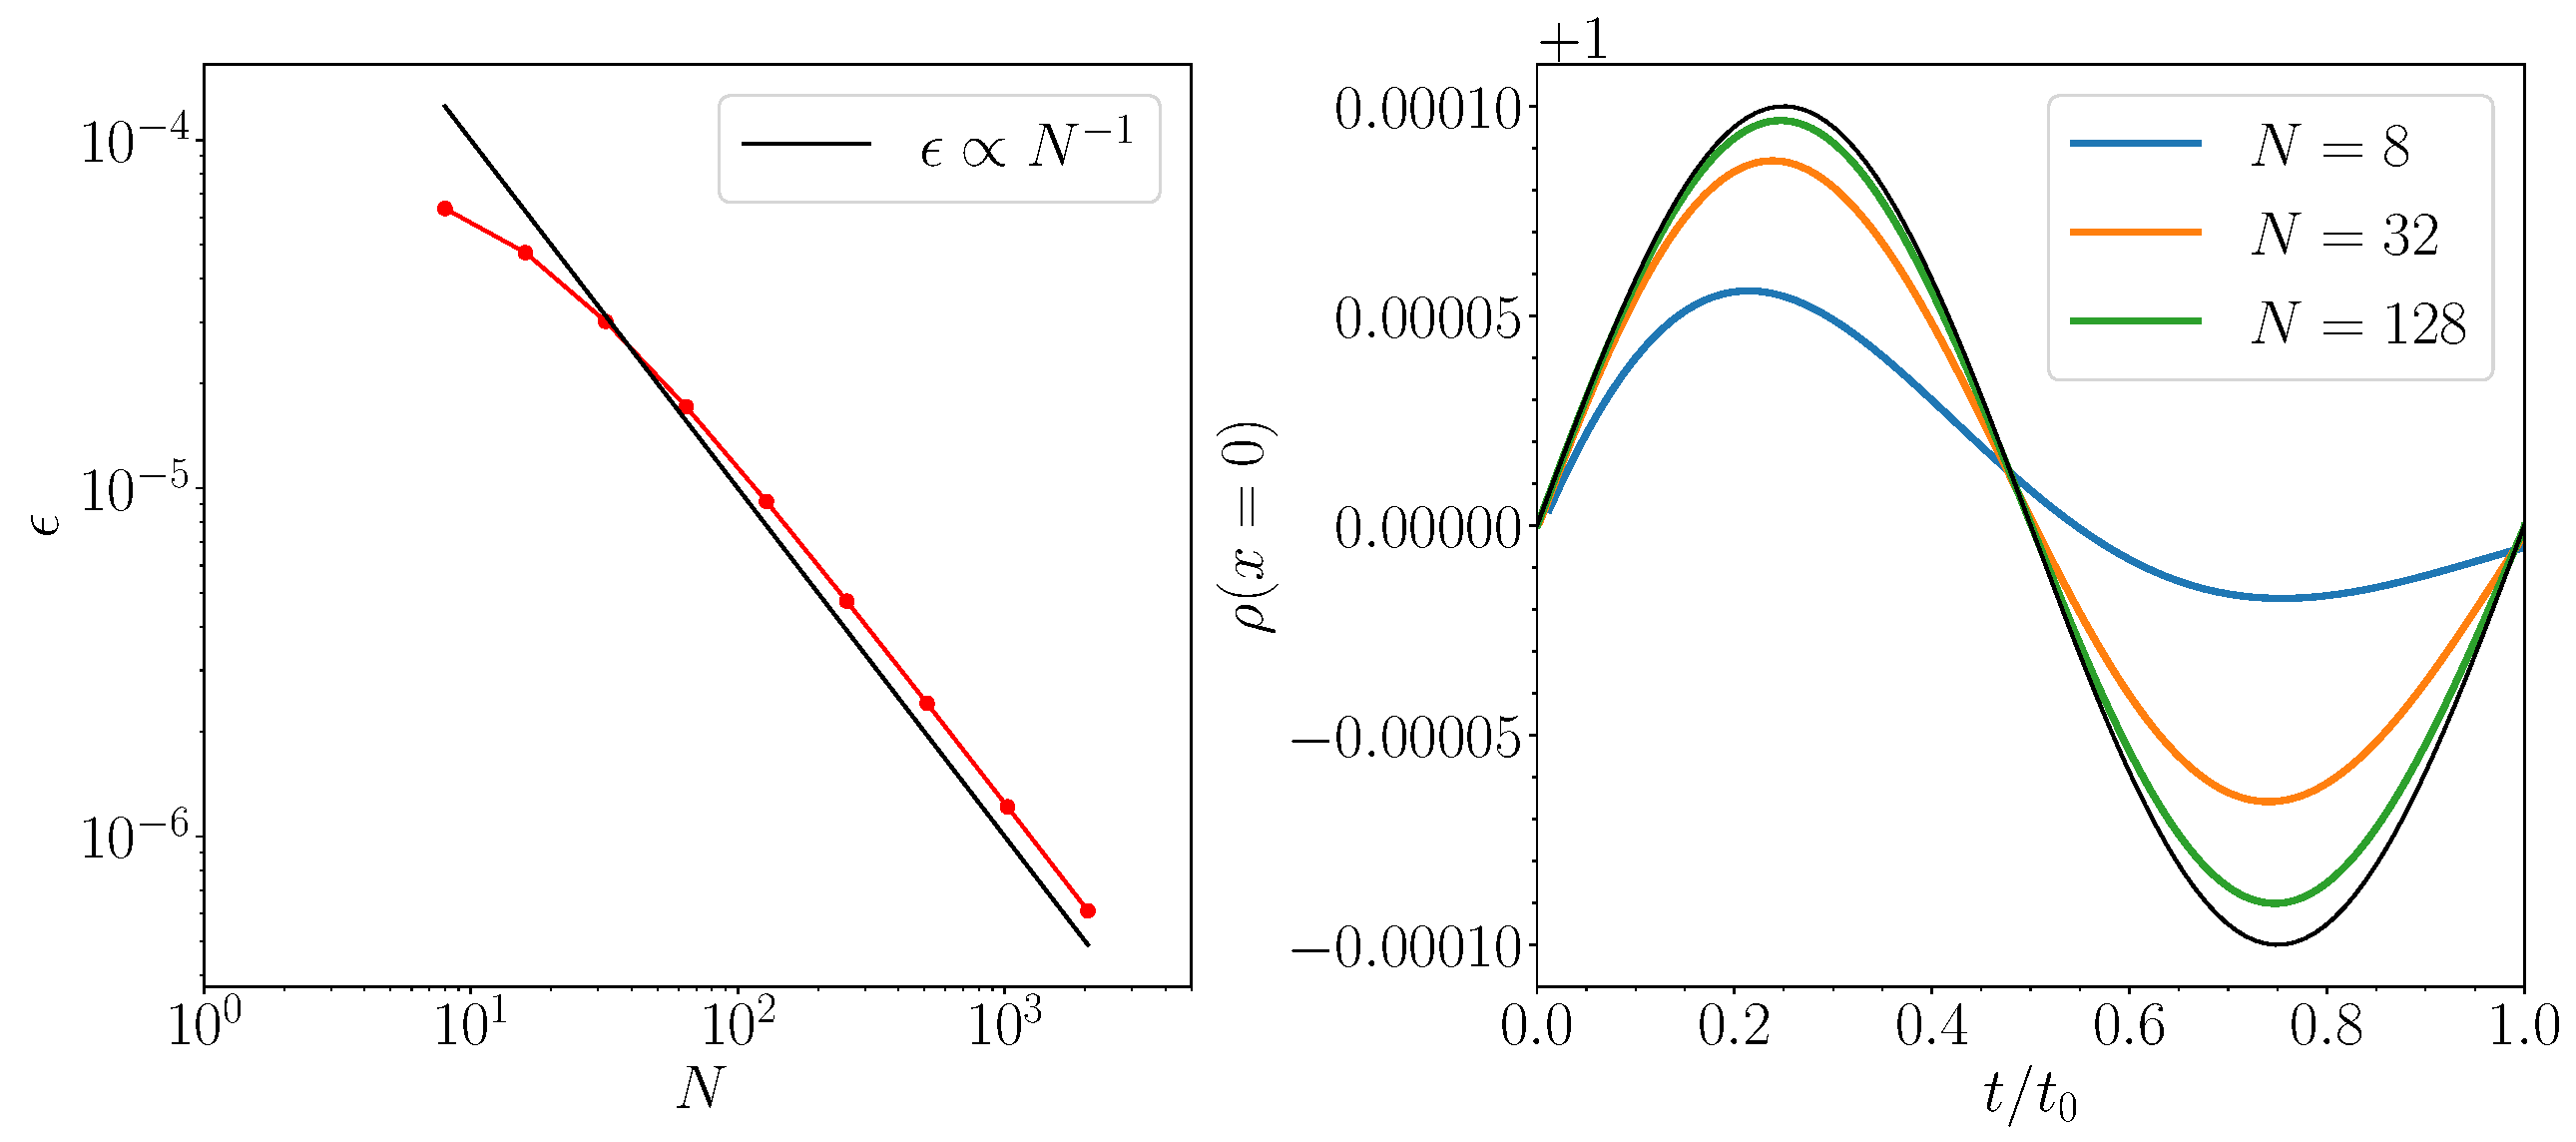
\includegraphics[width=16cm]{figures/sound.pdf}
    \caption{
    1次精度コードで音波を解いた結果。
    左:誤差の格子数依存性。右:$x=0$での密度の時間進化。
    }
    \label{fig:laxhllhllc}
\end{figure}

%------------------------------------------------------------
%------------------------------------------------------------
\clearpage
\section{磁気流体力学}
%------------------------------------------------------------
%------------------------------------------------------------

%------------------------------------------------------------
\subsection{Brio-Wu解 (1次元)}
%------------------------------------------------------------

%------------------------------------------------------------
\subsection{衝撃波管問題 in 2D}
%------------------------------------------------------------

以下の衝撃波管問題を考える。
添え字"1"と"2"は、初期不連続面に対して垂直成分と平行成分を表す。
初期条件を回転させる。
\begin{equation}
\left(
\begin{array}{c}
f_1 \\
f_2 \\
\end{array}
\right)
=
\left(
\begin{array}{cc}
\cos\alpha & - \sin\alpha \\
\sin\alpha & \cos\alpha \\
\end{array}
\right)
\left(
\begin{array}{c}
f_x \\
f_y \\
\end{array}
\right)
\end{equation}
回転角は$\alpha=\tan^{-1}2$とする($\cos\alpha=1/\sqrt{5}$,\;\;
$\sin\alpha=2/\sqrt{5}$)。初期不連続面は傾き$-1/2$の直線。

計算領域は$0\le x \le 1$、$0\le y \le 2/N_x$とする。
$y$方向はメッシュ数$2$。
$x$方向の境界条件はoutflowにする。
$y$方向の境界条件はoutflowにするが$x$方向にズラす。



\begin{equation}
\left(
\begin{array}{c}
\rho_\mathrm{L} \\
v_\mathrm{1,L} \\
v_\mathrm{2,L} \\
B_\mathrm{1,L} \\
B_\mathrm{2,L} \\
P_\mathrm{L} \\
\end{array}
\right)
= 
\left(
\begin{array}{c}
1 \\
10 \\
0 \\
5/\sqrt{4\pi} \\
5/\sqrt{4\pi} \\
20 \\
\end{array}
\right),\;\;\;
\left(
\begin{array}{c}
\rho_\mathrm{R} \\
v_\mathrm{1,R} \\
v_\mathrm{2,R} \\
B_\mathrm{1,R} \\
B_\mathrm{2,R} \\
P_\mathrm{R} \\
\end{array}
\right)
= 
\left(
\begin{array}{c}
1 \\
-10 \\
0 \\
5/\sqrt{4\pi} \\
5/\sqrt{4\pi} \\
1 \\
\end{array}
\right),\;\;\;
\label{shini}
\end{equation}



